\label{sec:householder}
\section{Linear algebra and indexing}

Modern numerical linear algebraists are used to writing expressions like:

\begin{itemize}

\item
The inner product of two vectors, $x^\prime y$, producing a scalar.

\item
The outer product of two vectors, $x y^\prime$, producing a matrix.

\item
Bilinear forms, $x^\prime A y$, and
quadratic/Hermitian forms, $x^\prime A y$, producing scalars.

\end{itemize}

These elementary forms can be used to construct much more complicated expressions, such as

\begin{itemize}

\item
Rayleigh quotients, $x^\prime A x / x^\prime x$,

\item
Updates to the quasi-Hessian in the Broyden--Fletcher--Goldfarb--Shanno (or BFGS) quasi-Newton algorithm, which take the form $\frac{x x^\prime}{x^\prime y} - \frac{A y y^\prime A}{y^\prime A y}$.

\item
The $F$-test statistic from linear hypothesis testing, which takes the form  $(Ax-y)^\prime (ABA^\prime)^{-1} (Ax-y)/\alpha$.

\end{itemize}

These expressions use Householder notation~\cite{Householder1953,Householder1955}, which used capital Roman letters for matrices, small Roman letters for (column) vectors, and small Greek letters for scalars.

We now argue that Householder notation was really meant for matrices, not scalars or vectors. If we use matrices in the expressions $U^\prime V$, $U V^\prime$ and $U^\prime A V$, then all these expressions can be defined with just matrix multiplication and matrix transposition. In fact, this is how Householder's seminal textbook on numerical computation defines vectors!\cite{Householder1955} Householder called $x$ and $y$ in these expressions ``numerical vectors'', which he identified with $n\times1$-matrices, as distinguished from
``geometrical vectors'', which are $n$-tuples with vector space structure.
If $x$ and $y$ were matrices, then the expressions for bilinear forms $x^\prime A y$ and inner products $x^\prime y$ can be evaluated using matrix multiplication and matrix transposition to produce $1\times1$ matrices. These resultant matrices are elements of $F^{1\times1}$, which is isomorphic to the field of zero-dimensional scalars $F$. In this sense, vectors in Householder notation are not ``flat'' $n$-tuples, but column vectors as shown in Figure~\ref{fig:zoo}. There are no true zero- or one-dimensional quantities in the universe described by Householder notation, only two-dimensional quantities whose names use capital Roman letters, small Roman letters or small Greek letters depending on how many dimensions are equal to 1.

Readers familiar with MATLAB will no doubt at this point be itching to point out MATLAB's automatic removal of trailing singleton dimensions in indexing expressions, which reads:

\begin{quote}
``MATLAB automatically removes trailing singleton dimensions (dimensions whose sizes are equal to 1) from all multidimensional arrays. For example, if you attempt to create an array of size 3-by-2-by-1-by-1, perhaps with the command \code{rand(3,2,1,1)}, then MATLAB strips away the singleton dimensions at the end of the array and creates a 3-by-2 matrix. This is because every array technically has an \textit{infinite} number of trailing singleton dimensions. A 3-by-2 array is the same as an array with size 3-by-2-by-1-by-1-by-1-by-...''--\cite{matlab.singleton}
\end{quote}

The trailing singleton dimensions rule allows MATLAB to identify $n\times1$ matrices with $n$-vectors, and $1\times1$ matrices with scalars, thus providing  the isomorphisms needed to produce scalars from $x^\prime A y$ and $x^\prime y$ while allowing one-dimensional indexing into the vectors $x$ and $y$. We believe it is no accident that MATLAB, the only language that has the trailing singleton dimensions rule for indexing, is also the only computer language designed from the very beginning for linear algebra.~\cite{Moler1980}

These identifications are also ubiquitous in the linear algebra literature; few authors bother to write out the isomorphisms explicitly. To give but one example, ``Lineare Algebra'' by Fischer, a well-known German text, writes

\begin{quote}
\[
(a_1...a_n) \cdot (b1 \vdots bn) = a_1 b_1 + \dots + a_n b_n \in K = M(1\times 1; K)
\]

,,In diesem Fall kann man $A$ und $B$ als Vektoren aus $K^n$ auffassen. Für $K=R$ ist dann $A\cdot B$ nichts anderes als das in (0.4.1) definiert Skalarproduct von $A$ und $B$.``

``In this case, one can regard $A$ and $B$ as vectors in $K^n$. For $K=R$ (the reals), $A\cdot B$ is none other than the scalar product of $A$ and
$B$ defined in (0.4.1).''

-\cite[p.\ 87]{Fischer1973}
\end{quote}

$K$ is the ring (,,Körper``) that is the underlying scalar field, and the equality $K = M(1\times 1; K)$ denotes the identification of the scalar field $K$ with $1\times 1$ matrices over $K$, $M(1\times 1; K)$ (which one might write as $K^{1\times1}$ in more contemporary notation). Two other authors notable for distinguishing carefully between $K$ and $K^{1\times1}$, and $K^{n\times1}$ and $K^n$ are Gantmacher\cite{Gantmacher1960} and Finkbeiner~\cite{Finkbeiner1960}.

The discussion of trailing singleton dimensions also makes clear that one of the fundamental distinctions between scalars, vectors and matrices are their abilities to be indexed into by zero, one and two indexes respectively.\footnote{Some languages like MATLAB support \textit{linear indexing}, where arrays of any rank can be indexed by one index. We ignore this complication here, focusing on simple indexing with Cartesian indexes.}
Thus it is their indexing behavior, specificially how many numbers are needed to label an element, that defines how scalars, vectors and matrices are said to be zero-, one- and two-dimensional objects respectively. In other words, scalars, vectors and matrices are arrays whose rank or dimensionality determines how many numbers are required to index an array element.


\subsection{A calculus for isomorphisms}

Let $F$ be a scalar field, $F^n$ be an $n$-dimensional vector space over $F$, and $F^{m\times n}$ be the set of $m\times n$-matrices over $F$.
Householder notation implicitly assumes a few embeddings,

\begin{enumerate}
\item
A $1\times1$ matrix is a scalar.
Give this embedding a name, $\theta:F^{1\times1}\rightarrow F$.

\item
An $n$-vector is an $n\times1$ matrix.
Give this embedding a name,
$\phi:F^n\rightarrow F^{n\times1}$.
\end{enumerate}

Figure~\ref{fig:embed} shows these embeddings $\theta$ and $\phi$ and how they are related to the menagerie of Figure~\ref{fig:zoo}.

\begin{figure}
\label{fig:embed}
\caption{Flat vectors vs row/column vectors and embeddings and transpositions.}

\centering{}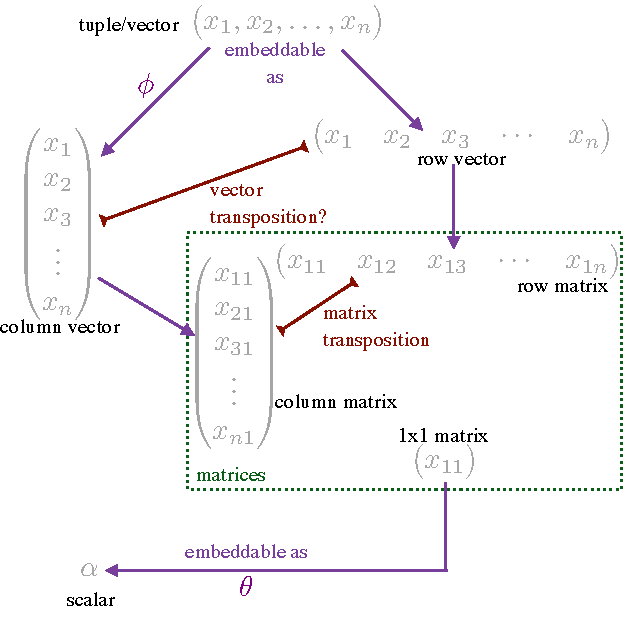
\includegraphics[width=0.9\columnwidth]{figures/fig-embed}
\end{figure}

Let's use these embeddings, and the identity embedding $I:F^{m\times n}\rightarrow F^{m\times n}$, to analyze the expressions listed at the beginning of Sec.~\ref{sec:householder}. Let $\circ$ denote composition of embeddings and operations like the matrix–matrix
product $*_{mm}:F^{m\times k}\times F^{k\times n}=F^{m\times n}$,
the matrix transpose $\cdot^\prime:F^{m\times n}\rightarrow F^{n\times m}$. Then:

\begin{itemize}
\item
The inner product $x^\prime y$ is the composition
$\theta\circ*_{mm}\circ\left(\cdot^\prime\times I\right)\circ\left(\phi\times\phi\right)$
acting on $(x,y)$.

\item
The outer product $xy^\prime$ is the composition
$*_{mm}\circ\left(I\times\cdot^{T}\right)\circ\left(\phi\times\phi\right)$
acting on $(x,y)$.

\item
The bilinear form $x^\prime Ay$, when evaluated in the order $x^\prime(Ay)$, is the composition
$\theta\circ*_{mm}\circ\left(\cdot^\prime\times*_{mm}\right)\circ\left(\phi\times I\times\phi\right)$ %
%
and when evaluated as $(x^\prime A)y$,
is the composition $\theta\circ*_{mm}\circ\left(*_{mm}\times I\right)\circ\left(\cdot^\prime\times I\times I\right)\circ\left(\phi\times I\times\phi\right)$,
%
both acting on $(x,A,y)$.
%
Some programming languages evaluate from left to right or from right to left.
Other programming languages (like C++) do not guarantee an evaluation order.
In these languages, for $x^\prime Ay$ to be well-defined regardless of the evaluation order, we must have the identity $*_{mm}\circ\left(\cdot^\prime\times*_{mm}\right)=\left(*_{mm}\times I\right)\circ\left(\cdot^\prime\times I\times I\right)$.
\end{itemize}

In these expressions, $\circ$ is function composition and $a\times b$
describes a sequence of operations $a$ and $b$ to be applied left
to right on a sequence of operands. $(I\times I)(A,B)$ means to apply
the identity map to $A$ and $B$ separately, producing the result
$(A,B)$. $(I\times*)(A,B,C)$ means to apply the identity map to
$A$ and the $*$ to the next two operands $B$ and $C$ (since $I$
is monadic and $*$ is dyadic), producing the result $(A,BC)$.

This section was about defining platonic ideal semantics. In Sec.~\ref{sec:reallanguages}, we will see how real programming languages complicate the picture, namely the limitations of working only at the individual operator level and not at the whole-expression level.
